\section{Описание алгоритма}
    На $k$-том шаге в необработанных до этого строках системы находится максимальный по модулю элемент. Пусть это будет элемент $a_{ij}$. Из каждой другой необработанной $l$-той строки вычитается данная строка, умноженная на $\frac{a_{lj}}{a_{ij}}$, тем самым получая нули в $j$-том столбце данных строк.

    После $n-1$ шага получается матрица, которую можно решить путём исключения переменных.

\section{Код}
    \href{https://github.com/Dezzelshipc/CompMath/blob/main/sem5-compmath/lab2.py}{Ссылка на код.}

\pagebreak

\section{Тестирование}
    \begin{figure}[H]
        \centering
        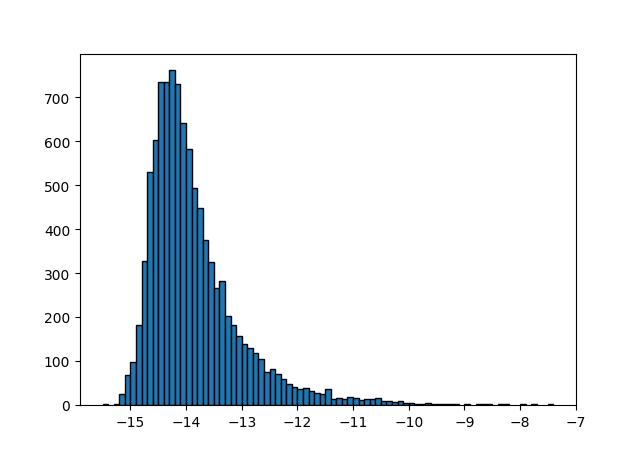
\includegraphics[width=16cm]{pictures/BarCounts.png}
        \caption{Log10 максимальной разницы решения алгоритма и встроенной функции numpy, округлённый до десятых при генерации 10000 случайных матриц.}
    \end{figure}

    На рисунке 1 можно увидеть распределения точностей решения. Большинство решений по точности не превышает $10^{-10}$. Решения с меньшей точностью определяются большим числом обусловленности сгенерированной матрицы -- от 2000 до 31000. Однако, количество таких решений -- $29$, что составляет всего $0.29 \% $ от всех решений.

    \begin{figure}[H]
        \centering
        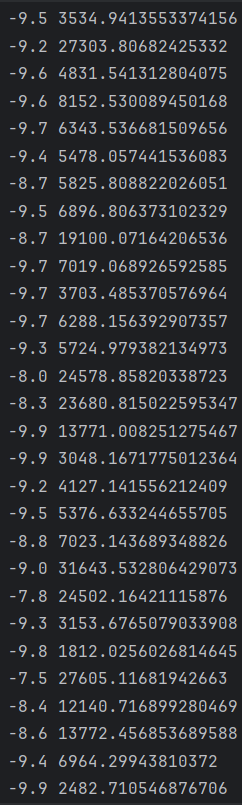
\includegraphics[width=6cm]{pictures/BigConditions.png}
        \caption{Log10 разности и число обусловленности решений, которые не превысили точность $10^{-10}$.}
    \end{figure}